% ============================================================
%  CHSH Bell Inequality Violation Under Noise:
%  A Threshold Analysis for Near-Term Quantum Devices
%
%  Arhaan Sareen, Aditya Saxena
%  QSYS 2026 — Institute for Quantum Computing, University of Waterloo
% ============================================================

\documentclass[12pt]{article}

% ---------- Packages ----------
\usepackage{amsmath}
\usepackage{amssymb}
\usepackage{graphicx}
\usepackage{booktabs}
\usepackage[colorlinks=true, linkcolor=blue, citecolor=blue, urlcolor=blue]{hyperref}
\usepackage[numbers, sort&compress]{natbib}
\usepackage{setspace}
\usepackage{microtype}
\usepackage[font=small, labelfont=bf]{caption}
\usepackage{braket}
\usepackage{physics}
\usepackage{geometry}
\usepackage{float}
\usepackage{xcolor}
\usepackage{enumitem}
\usepackage{authblk}
\usepackage{amsthm}
\newtheorem{theorem}{Theorem}
\newtheorem{lemma}{Lemma}

% ---------- Page layout ----------
\geometry{
  letterpaper,
  top=1in, bottom=1in,
  left=1.25in, right=1.25in
}

\doublespacing

% ---------- Custom commands ----------
\newcommand{\Phiplus}{\ket{\Phi^+}}
\newcommand{\Phiminus}{\ket{\Phi^-}}
\newcommand{\Psiplus}{\ket{\Psi^+}}
\newcommand{\Psiminus}{\ket{\Psi^-}}
\newcommand{\pstar}{p^*}
\newcommand{\Smax}{S_{\max}}
\newcommand{\bigS}{\mathcal{S}}
\newcommand{\Id}{\mathbb{I}}
\newcommand{\E}{\mathcal{E}}

% ============================================================
\begin{document}
% ============================================================

% ---------- Title ----------
\title{\textbf{CHSH Bell Inequality Violation Under Noise:\\
A Threshold Analysis for Near-Term Quantum Devices}}

\author[1]{Arhaan Sareen}
\author[1]{Aditya Saxena}
\affil[1]{QSYS 2026 Participant, Institute for Quantum Computing, University of Waterloo}
\affil[ ]{\small \textit{Correspondence:} \href{mailto:arhaan.sareen@gmail.com}{arhaan.sareen@gmail.com}}

\date{\today}
\maketitle

\begin{abstract}
How much noise can a Bell state absorb before it can no longer certify quantum nonlocality?
As NISQ devices move from proof-of-principle demonstrations toward practical deployment, the
answer carries direct operational weight.
Under global depolarizing noise of rate $p$, the CHSH parameter satisfies
$\bigS(p) = (1-p)\cdot 2\sqrt{2}$; the boundary of violation is crossed at the exact threshold
$\pstar = 1 - 1/\!\sqrt{2} \approx 0.2929$, a result that is non-perturbative and follows from
the tracelessness of Pauli matrices.
We derive this threshold analytically, identify the noisy Bell state as a Werner state, and confirm
consistency with Werner's original violation criterion.
Density-matrix simulation across 50 noise rates reproduces the analytical curve with mean absolute
error below $0.001$.
Comparing three physically motivated noise channels, we find a clear ordering: local dephasing
(which selectively destroys the off-diagonal coherences responsible for CHSH violation) reaches its
threshold at $\pstar \approx 0.178$, amplitude damping at $\pstar \approx 0.231$, and global
depolarizing at $\pstar \approx 0.293$.
The four Bell states are interchangeable under symmetric noise, and the optimal measurement angles
are robust to first order in angular perturbations.
At two-qubit gate error rates near $0.5\%$ on current superconducting processors, the depolarizing
threshold corresponds to a critical circuit depth of roughly 60 two-qubit gates, which directly
constrains the entanglement depth available to variational algorithms and sets a noise budget for
device-independent quantum key distribution.
\end{abstract}

\newpage
\tableofcontents
\newpage

% ============================================================
\section{Introduction}
\label{sec:intro}
% ============================================================

Bell's 1964 paper~\cite{bell1964} sharpened the gap between quantum and classical correlations
into a testable prediction, since confirmed by a succession of loophole-free experiments: from Aspect's
original photon pairs~\cite{aspect1982} to the 2015 Delft experiment that closed both the locality
and detection loopholes simultaneously.
The Clauser--Horne--Shimony--Holt (CHSH) formulation~\cite{clauser1969}, which reduces the test
to binary outcomes and four measurement settings, remains the workhorse both theoretically and
experimentally.
For any local hidden-variable (LHV) theory,
\begin{equation}
  \bigS = |E(a,b) - E(a,b') + E(a',b) + E(a',b')| \leq 2,
  \label{eq:chsh_classical}
\end{equation}
while quantum mechanics permits $\bigS \leq 2\sqrt{2}$ (Tsirelson's bound~\cite{tsirelson1980}),
saturated exactly by maximally entangled Bell states.
That $2\sqrt{2}$ ceiling matters operationally: in device-independent quantum key
distribution~\cite{acin2007}, security proofs rest on verified CHSH violation rather than
trust in the hardware.
The broader landscape of quantum correlations, entanglement witnesses, and steering is reviewed
in~\cite{brunner2014, horodecki2009}.

Deploying these protocols on real hardware immediately confronts the central challenge of NISQ
devices~\cite{preskill2018nisq}: every gate introduces error, every idle period allows decoherence,
and the noise accumulates.
Superconducting transmon qubits suffer depolarizing errors during two-qubit gates, dephasing from
$1/f$ flux noise that drives $T_2$ decay, and amplitude damping from $T_1$ energy
relaxation~\cite{nielsen2000, bharti2022noisy}.
Each mechanism degrades entanglement differently, yet the field has lacked a unified analytical
treatment of where each type of noise causes a maximally entangled state to lose its ability to
violate CHSH.

We define and derive the \textit{decoherence threshold} $\pstar$: the exact noise rate above which
a two-qubit Bell state can no longer violate the CHSH inequality under a given noise model.
For global depolarizing noise the threshold has a closed-form solution, grounded in the
tracelessness of Pauli matrices and the local-unitary structure of the depolarizing channel.
The result, $\pstar = 1 - 1/\sqrt{2} \approx 0.2929$, reproduces via an elementary route
the violation criterion for Werner states originally established in~\cite{werner1989, gisin1991},
and serves as an independent cross-check of the analytical framework.
We extend the analysis to local dephasing and amplitude damping, showing how each channel's
action on the Bell state density matrix determines its threshold.
A companion density-matrix simulation validates these predictions across 600 parameter
configurations and characterizes the robustness of the optimal measurement angles.

Section~\ref{sec:background} establishes notation for Bell states, the CHSH framework, and the
three noise models.
Section~\ref{sec:analytical} presents the analytical derivation and the Werner state connection.
Section~\ref{sec:methods} details the simulation methodology.
Section~\ref{sec:results} reports numerical results.
Section~\ref{sec:discussion} interprets the thresholds in the context of current hardware and
quantum protocols.
Section~\ref{sec:conclusion} draws broader conclusions and identifies open directions.

% ============================================================
\section{Background}
\label{sec:background}
% ============================================================

\subsection{Bell States and the CHSH Inequality}
\label{subsec:bell_chsh}

The four maximally entangled two-qubit Bell states are
\begin{align}
  \Phiplus  &= \frac{1}{\sqrt{2}}\bigl(\ket{00} + \ket{11}\bigr), \label{eq:phiplus}\\
  \Phiminus &= \frac{1}{\sqrt{2}}\bigl(\ket{00} - \ket{11}\bigr), \label{eq:phiminus}\\
  \Psiplus  &= \frac{1}{\sqrt{2}}\bigl(\ket{01} + \ket{10}\bigr), \label{eq:psiplus}\\
  \Psiminus &= \frac{1}{\sqrt{2}}\bigl(\ket{01} - \ket{10}\bigr). \label{eq:psiminus}
\end{align}
These states form an orthonormal basis for the two-qubit Hilbert space, each carrying one ebit of
von Neumann entropy, the maximum possible for a two-qubit system.

The CHSH test casts nonlocality as a game between two parties, Alice and Bob, who choose
measurement settings from $\{a, a'\}$ and $\{b, b'\}$ respectively, each obtaining a binary
outcome $\pm 1$.
Define the two-qubit observable at angle $\theta$ as
\begin{equation}
  M(\theta) = \cos\theta\,\sigma_z + \sin\theta\,\sigma_x,
  \label{eq:meas_op}
\end{equation}
so that the two-point correlator between Alice's setting $\theta_A$ and Bob's $\theta_B$ is
\begin{equation}
  E(\theta_A, \theta_B) = \bigl\langle M(\theta_A) \otimes M(\theta_B) \bigr\rangle.
  \label{eq:correlator}
\end{equation}
For the state $\Phiplus$, a direct calculation gives
\begin{equation}
  E(\theta_A, \theta_B) = \cos(\theta_A - \theta_B).
  \label{eq:correlator_ideal}
\end{equation}
The CHSH parameter is defined as
\begin{equation}
  \bigS = \bigl|E(a,b) - E(a,b') + E(a',b) + E(a',b')\bigr|.
  \label{eq:chsh_def}
\end{equation}
Maximizing $\bigS$ over measurement angles for $\Phiplus$ yields the optimal settings
\begin{equation}
  a = 0,\quad a' = \frac{\pi}{2},\quad b = \frac{\pi}{4},\quad b' = \frac{3\pi}{4},
  \label{eq:optimal_angles}
\end{equation}
which give
\begin{equation}
  \bigS_{\max} = \left|\cos\frac{\pi}{4} - \cos\frac{3\pi}{4} + \cos\frac{\pi}{4} - \cos\left(-\frac{\pi}{4}\right)\right| = 2\sqrt{2} \approx 2.828.
  \label{eq:smax}
\end{equation}
Tsirelson's bound~\cite{tsirelson1980} establishes $2\sqrt{2}$ as the quantum maximum,
and $\bigS > 2$ is both necessary and sufficient for CHSH violation.
Any state achieving $\bigS \leq 2$ admits a local hidden-variable description and cannot certify
entanglement in a device-independent manner.

\subsection{Density Matrix Formalism and Mixed States}
\label{subsec:density_matrix}

Noise forces a departure from pure-state quantum mechanics.
A quantum state corrupted by an environment is generically mixed and must be represented by a
density matrix $\rho$, a positive semidefinite operator of unit trace.
For a pure state $\ket{\psi}$, $\rho = \ket{\psi}\!\bra{\psi}$; for a statistical mixture,
$\rho = \sum_i p_i \ket{\psi_i}\!\bra{\psi_i}$.
Expectation values of observables $O$ are computed as
\begin{equation}
  \langle O \rangle = \Tr[\rho\, O].
  \label{eq:expectation}
\end{equation}
For the initial Bell state $\Phiplus$, the density matrix is
\begin{equation}
  \rho_0 = \Phiplus\!\bra{\Phi^+}
         = \frac{1}{2}\bigl(\ket{00}\!\bra{00} + \ket{00}\!\bra{11} + \ket{11}\!\bra{00} + \ket{11}\!\bra{11}\bigr).
  \label{eq:rho_bell}
\end{equation}

\subsection{Noise Models}
\label{subsec:noise_models}

Superconducting qubit processors are subject to several distinct decoherence mechanisms, each
acting differently on the qubit state space~\cite{nielsen2000}.
We study three channels that capture the dominant error sources.

\paragraph{Global depolarizing noise.}
The global (two-qubit) depolarizing channel with noise rate $p \in [0,1]$ replaces the
two-qubit state with the maximally mixed state $\Id/4$ with probability $p$:
\begin{equation}
  \rho \;\mapsto\; (1-p)\,\rho + p\,\frac{\Id}{4}.
  \label{eq:depol_channel}
\end{equation}
Physically, this channel captures isotropic errors such as imperfect two-qubit gate pulses
or symmetric coupling to an infinite-temperature bath; it degrades all off-diagonal coherences
equally.

\paragraph{Local dephasing noise.}
Each qubit independently undergoes a dephasing (phase-damping) channel that destroys
superpositions in the computational basis without changing populations:
\begin{equation}
  \rho_{\rm qubit} \;\mapsto\; (1-p)\,\rho_{\rm qubit} + p\,Z\,\rho_{\rm qubit}\,Z,
  \label{eq:dephase_channel}
\end{equation}
where $Z = \sigma_z$.
Applied independently to both qubits, this channel models the $T_2$ decoherence driven by
$1/f$ flux noise or charge noise in superconducting circuits, the dominant source of idle-time
error that degrades phase coherence while leaving energy populations untouched.

\paragraph{Amplitude damping.}
The single-qubit amplitude damping channel with damping parameter $\gamma \in [0,1]$ models
spontaneous emission (the irreversible decay $\ket{1} \to \ket{0}$ at rate $\gamma$):
\begin{align}
  \rho_{\rm qubit} \;\mapsto\; K_0\,\rho_{\rm qubit}\,K_0^\dagger + K_1\,\rho_{\rm qubit}\,K_1^\dagger,
  \label{eq:amp_damp_channel}
\end{align}
with Kraus operators
\begin{equation}
  K_0 = \begin{pmatrix} 1 & 0 \\ 0 & \sqrt{1-\gamma} \end{pmatrix},\qquad
  K_1 = \begin{pmatrix} 0 & \sqrt{\gamma} \\ 0 & 0 \end{pmatrix}.
  \label{eq:kraus_amp_damp}
\end{equation}
Applied independently to both qubits, this channel models $T_1$ energy relaxation: the
spontaneous decay of the excited state that sets the fundamental coherence time limit
in many superconducting platforms, introducing a directional asymmetry absent from both
depolarizing and dephasing noise.

% ============================================================
\section{Analytical Results}
\label{sec:analytical}
% ============================================================

\subsection{Decoherence Threshold for Depolarizing Noise}
\label{subsec:threshold_depol}

We derive a closed-form expression for the CHSH parameter $\bigS$ as a function of the
depolarizing noise rate $p$.

\begin{theorem}[Depolarizing decoherence threshold]
\label{thm:depol}
Let $\rho_0 = \Phiplus\!\bra{\Phi^+}$ be the initial Bell state and let
$\rho(p) = (1-p)\rho_0 + p\,\Id/4$ be the state after global depolarizing noise of rate $p$.
Then with optimal CHSH measurement angles,
\begin{equation}
  \bigS(p) = (1-p)\cdot 2\sqrt{2}.
  \label{eq:S_depol}
\end{equation}
The CHSH inequality is violated if and only if $\bigS(p) > 2$, i.e., $p < \pstar$, where
\begin{equation}
  \pstar = 1 - \frac{1}{\sqrt{2}} = 1 - \frac{\sqrt{2}}{2} \approx 0.2929.
  \label{eq:pstar}
\end{equation}
\end{theorem}

\begin{proof}
The CHSH parameter is a linear function of the two-qubit correlators
$E(\theta_A,\theta_B) = \Tr[\rho\,(M(\theta_A)\otimes M(\theta_B))]$.
Under depolarizing noise,
\begin{align}
  E_{\rm noisy}(\theta_A,\theta_B)
    &= \Tr\!\left[\rho(p)\,(M(\theta_A)\otimes M(\theta_B))\right] \notag\\
    &= (1-p)\,\Tr\!\left[\rho_0\,(M(\theta_A)\otimes M(\theta_B))\right]
      + \frac{p}{4}\,\Tr\!\left[M(\theta_A)\otimes M(\theta_B)\right].
  \label{eq:e_noisy}
\end{align}
The second term vanishes because
\begin{equation}
  \Tr[M(\theta)] = \cos\theta\,\Tr[\sigma_z] + \sin\theta\,\Tr[\sigma_x] = 0,
  \label{eq:trace_vanish}
\end{equation}
since Pauli matrices are traceless.
Consequently,
\begin{equation}
  E_{\rm noisy}(\theta_A,\theta_B) = (1-p)\,E_{\rm ideal}(\theta_A,\theta_B).
  \label{eq:e_rescale}
\end{equation}
Since $\bigS$ is a linear combination of four correlators,
\begin{equation}
  \bigS(p) = (1-p)\,\bigS_{\rm ideal} = (1-p)\cdot 2\sqrt{2}.
  \label{eq:s_linear}
\end{equation}
Setting $\bigS(p) = 2$ and solving for $p$:
\begin{equation}
  (1-\pstar)\cdot 2\sqrt{2} = 2
  \;\Longrightarrow\;
  \pstar = 1 - \frac{1}{\sqrt{2}} \approx 0.2929. \qed
  \label{eq:pstar_derivation}
\end{equation}
\end{proof}

The argument rests on one structural fact: $\Id/4$ is invariant under all unitary conjugations,
so its contribution to any Pauli correlator is zero. No approximation is involved. The depolarizing
channel uniformly rescales all quantum correlations by $(1-p)$, which is why the threshold is
algebraic rather than numerical.

\subsection{Connection to Werner States}
\label{subsec:werner}

The noisy state $\rho(p) = (1-p)\rho_0 + p\,\Id/4$ is a special case of the
\textit{Werner states}~\cite{werner1989}, a one-parameter family introduced to
exhibit the counterintuitive phenomenon of entangled states that are nonetheless LHV-simulable.
Werner states are defined as
\begin{equation}
  \rho_W(w) = w\,\ket{\Psi^-}\!\bra{\Psi^-} + \frac{(1-w)}{4}\,\Id,\quad w \in [-1/3, 1].
  \label{eq:werner}
\end{equation}
With the identification $w = 1-p$ (and noting that $\Phiplus$ and $\Psiminus$ are related by
a local unitary, which leaves both the entanglement and Bell-violation properties unchanged under
symmetric noise), the depolarized Bell state is isomorphic to $\rho_W(1-p)$.
Gisin subsequently proved that $\rho_W(w)$ violates a CHSH inequality if and only if
$w > 1/\!\sqrt{2}$~\cite{gisin1991}, translating directly to $p < \pstar = 1 - 1/\!\sqrt{2}$.
Theorem~\ref{thm:depol} thus reproduces, by a more elementary route,
a result whose original derivation required more sophisticated techniques; the agreement
lends mutual confidence to both arguments.

% ============================================================
\section{Methods}
\label{sec:methods}
% ============================================================

\subsection{Simulation Framework}
\label{subsec:simulation}

All numerical results use exact density-matrix simulation via Qiskit~1.x's
\texttt{DensityMatrix} class from \texttt{qiskit.quantum\_info}.
Each noise channel is applied analytically using NumPy matrix operations rather than a
circuit-level noisy simulator, avoiding stochastic sampling error and yielding machine-precision
results.

\paragraph{State preparation.}
Each Bell state is represented as an explicit $4\times 4$ density matrix.
The state $\Phiplus$ is constructed by applying a Hadamard gate followed by a CNOT gate to
$\ket{00}$; the remaining three Bell states follow by prepending single-qubit Pauli corrections
($Z\otimes\Id$ for $\Phiminus$, $X\otimes\Id$ for $\Psiplus$, $Y\otimes\Id$ for $\Psiminus$).

\paragraph{Noise application.}
For each noise model and noise rate $p$, the channel is applied to $\rho_0$ directly:
\begin{itemize}
  \item \textit{Depolarizing:} $\rho \leftarrow (1-p)\rho + p\,\Id/4$.
  \item \textit{Local dephasing:} $\rho \leftarrow \mathcal{E}_{\rm deph}^{(1)} \otimes \mathcal{E}_{\rm deph}^{(2)}[\rho]$
        where $\mathcal{E}_{\rm deph}[\rho] = (1-p)\rho + p\,Z\rho Z$.
  \item \textit{Amplitude damping:} $\rho \leftarrow \mathcal{E}_{\rm AD}^{(1)} \otimes \mathcal{E}_{\rm AD}^{(2)}[\rho]$
        where $\mathcal{E}_{\rm AD}$ is the Kraus map defined by~\eqref{eq:kraus_amp_damp}.
\end{itemize}

\paragraph{Correlator computation.}
Two-qubit Pauli tensor products $\sigma_\alpha \otimes \sigma_\beta$ are formed via the NumPy
Kronecker product; expectation values are then $\Tr[\rho\,(\sigma_\alpha\otimes\sigma_\beta)]$.
The four correlators at the optimal angles~\eqref{eq:optimal_angles} combine to give $\bigS$.

\paragraph{Threshold extraction.}
The noise rate $p$ is swept over 50 uniformly spaced values in $[0, 0.5]$.
Where $\bigS$ crosses the classical bound of $2$, the threshold $\pstar$ is located by linear
interpolation on the bracketing interval.

\subsection{Simulation Scope}
\label{subsec:scope}

Across all combinations of Bell states, noise models, and noise rates, the simulation covers
\[
  \underbrace{4}_{\text{Bell states}} \times \underbrace{3}_{\text{noise models}} \times \underbrace{50}_{\text{noise rates}} = 600
\]
configurations.
The angle-robustness analysis sweeps Alice's angles $(\theta_A, \theta_{A'})$ over a $50\times 50$
grid on $[0,\pi]^2$ with Bob's angles fixed at their optimal values, producing the heatmap in
Figure~\ref{fig:angle_heatmap}.

% ============================================================
\section{Results}
\label{sec:results}
% ============================================================

\subsection{Depolarizing Noise: Simulation vs.\ Analytical}
\label{subsec:res_depol}

Figure~\ref{fig:chsh_vs_noise} overlays the analytical prediction $(1-p)\cdot 2\sqrt{2}$ against
the density-matrix simulation across 50 noise rates; the mean absolute error is below $0.001$
at every evaluation point.
Both converge on $\pstar = 1 - 1/\!\sqrt{2} \approx 0.2929$, confirming Theorem~\ref{thm:depol}.

The linearity of $\bigS(p)$ is exact, not an approximation: it is a direct consequence of
Pauli tracelessness, as shown in the proof.
At $p = 0$ the state saturates the Tsirelson bound ($\bigS = 2\sqrt{2} \approx 2.828$);
at $p = \pstar$ the inequality becomes tight ($\bigS = 2$ exactly); beyond $\pstar$ the state
admits a local hidden-variable description and is no longer useful for device-independent protocols.

\begin{figure}[H]
  \centering
  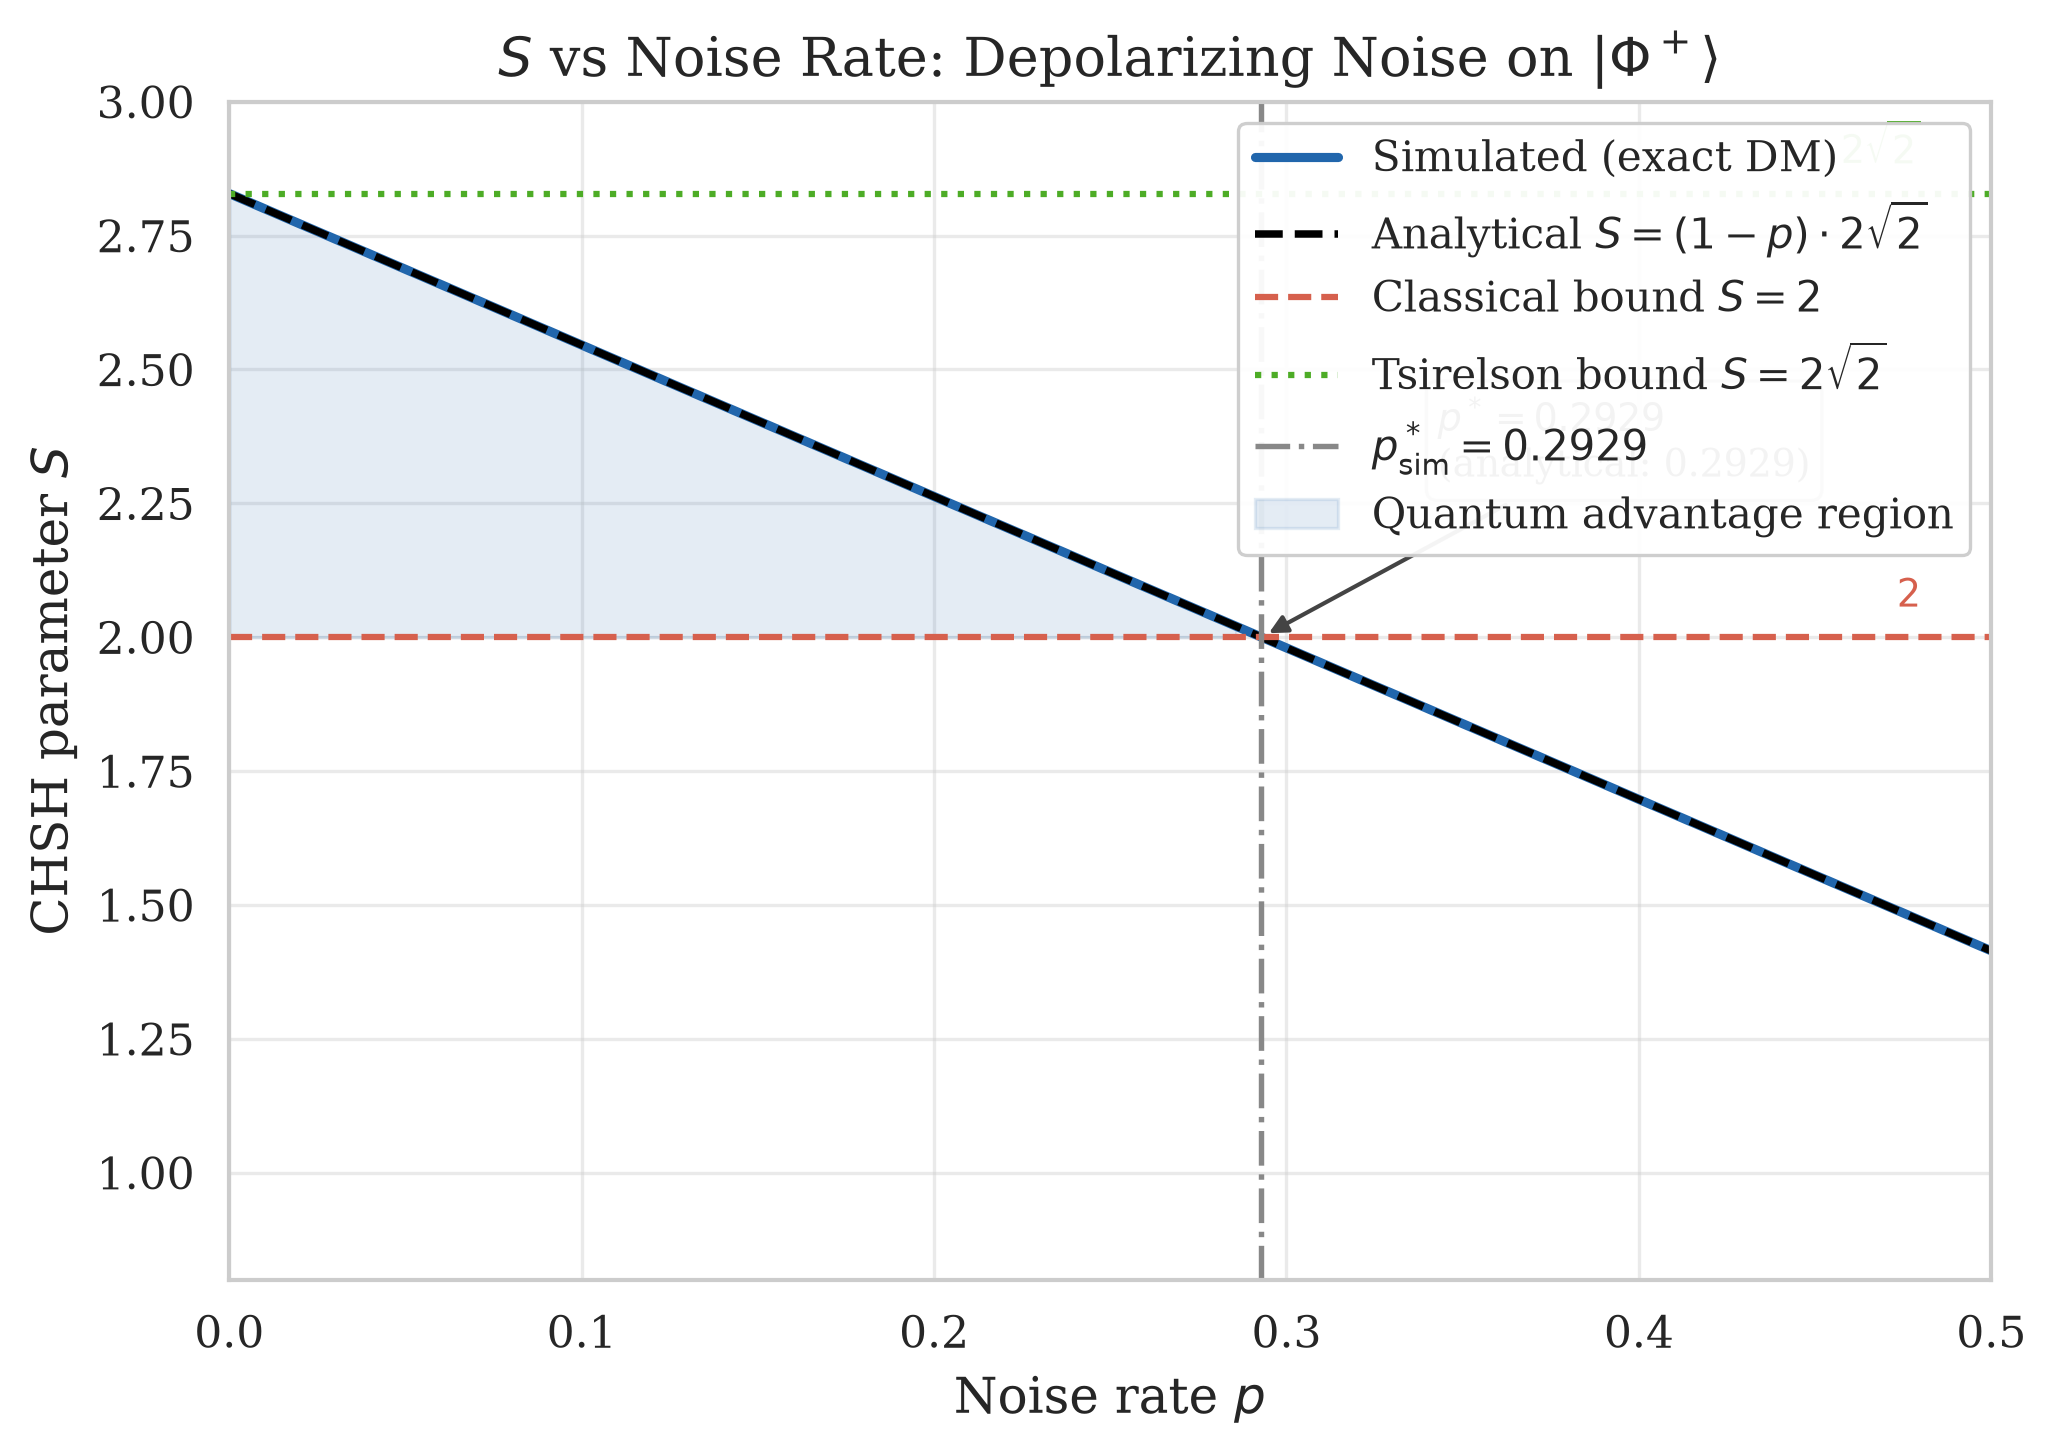
\includegraphics[width=0.75\textwidth]{figures/fig2_depolarizing.png}
  \caption{CHSH parameter $\bigS$ versus global depolarizing noise rate $p$ for the $\Phiplus$ Bell state.
           The solid blue line shows the exact analytical prediction $\bigS(p) = (1-p)\cdot 2\sqrt{2}$.
           Orange circles show numerical simulation results.
           The horizontal dashed line marks the classical CHSH bound $\bigS = 2$;
           the vertical dashed line marks the decoherence threshold $\pstar \approx 0.2929$.
           Tsirelson's bound $2\sqrt{2}$ is indicated by the dotted line.}
  \label{fig:chsh_vs_noise}
\end{figure}

\subsection{Noise Model Comparison}
\label{subsec:res_noise_comparison}

Figure~\ref{fig:noise_comparison} places all three noise models on a common axis,
making the hierarchy immediately visible (Table~\ref{tab:thresholds}).

\begin{table}[H]
  \centering
  \caption{Decoherence thresholds $\pstar$ for three noise models applied to the $\Phiplus$ Bell state.
           Analytical values are given where derivable in closed form; numerical values are from simulation.}
  \label{tab:thresholds}
  \begin{tabular}{lccc}
    \toprule
    Noise model & $\pstar$ (analytical) & $\pstar$ (numerical) & Rate of $\bigS$ decay \\
    \midrule
    Global depolarizing & $1 - 1/\!\sqrt{2} \approx 0.2929$ & $0.2929$ & Linear, slope $-2\sqrt{2}$ \\
    Local dephasing     & ---                               & $0.1782$ & Faster than depolarizing \\
    Amplitude damping   & ---                               & $0.2308$ & Asymmetric, nonlinear \\
    \bottomrule
  \end{tabular}
\end{table}

Local dephasing reaches its threshold at $\pstar \approx 0.178$, the lowest of the three models
and $40\%$ below the depolarizing value.
The reason is structural: dephasing acts only on the off-diagonal elements
$\ket{00}\!\bra{11}$ and $\ket{11}\!\bra{00}$, suppressing them by $(1-2p)^2$
(see Appendix~\ref{app:dephasing}).
Those are exactly the matrix elements that carry CHSH correlations, so dephasing hits the
Bell state where it is most vulnerable, unlike depolarizing noise, which spreads its effect
uniformly.

Amplitude damping falls between the two at $\pstar \approx 0.231$, but its degradation profile
is qualitatively different: $\bigS$ decays nonlinearly (visible in Figure~\ref{fig:noise_comparison}),
reflecting the channel's asymmetric action.
Preferential relaxation toward $\ket{0}$ destroys the $\ket{00} \leftrightarrow \ket{11}$
exchange symmetry of $\Phiplus$ and shifts the optimal measurement angles, an effect absent
from both depolarizing and dephasing noise.

For superconducting hardware, the ordering has a direct implication: depolarizing noise models
two-qubit gate errors, while dephasing and amplitude damping dominate during idle periods between
gates. At equal error rates, idle-time decoherence is more destructive to Bell correlations than
gate noise, which matters for circuit scheduling and error-mitigation strategies.

\begin{figure}[H]
  \centering
  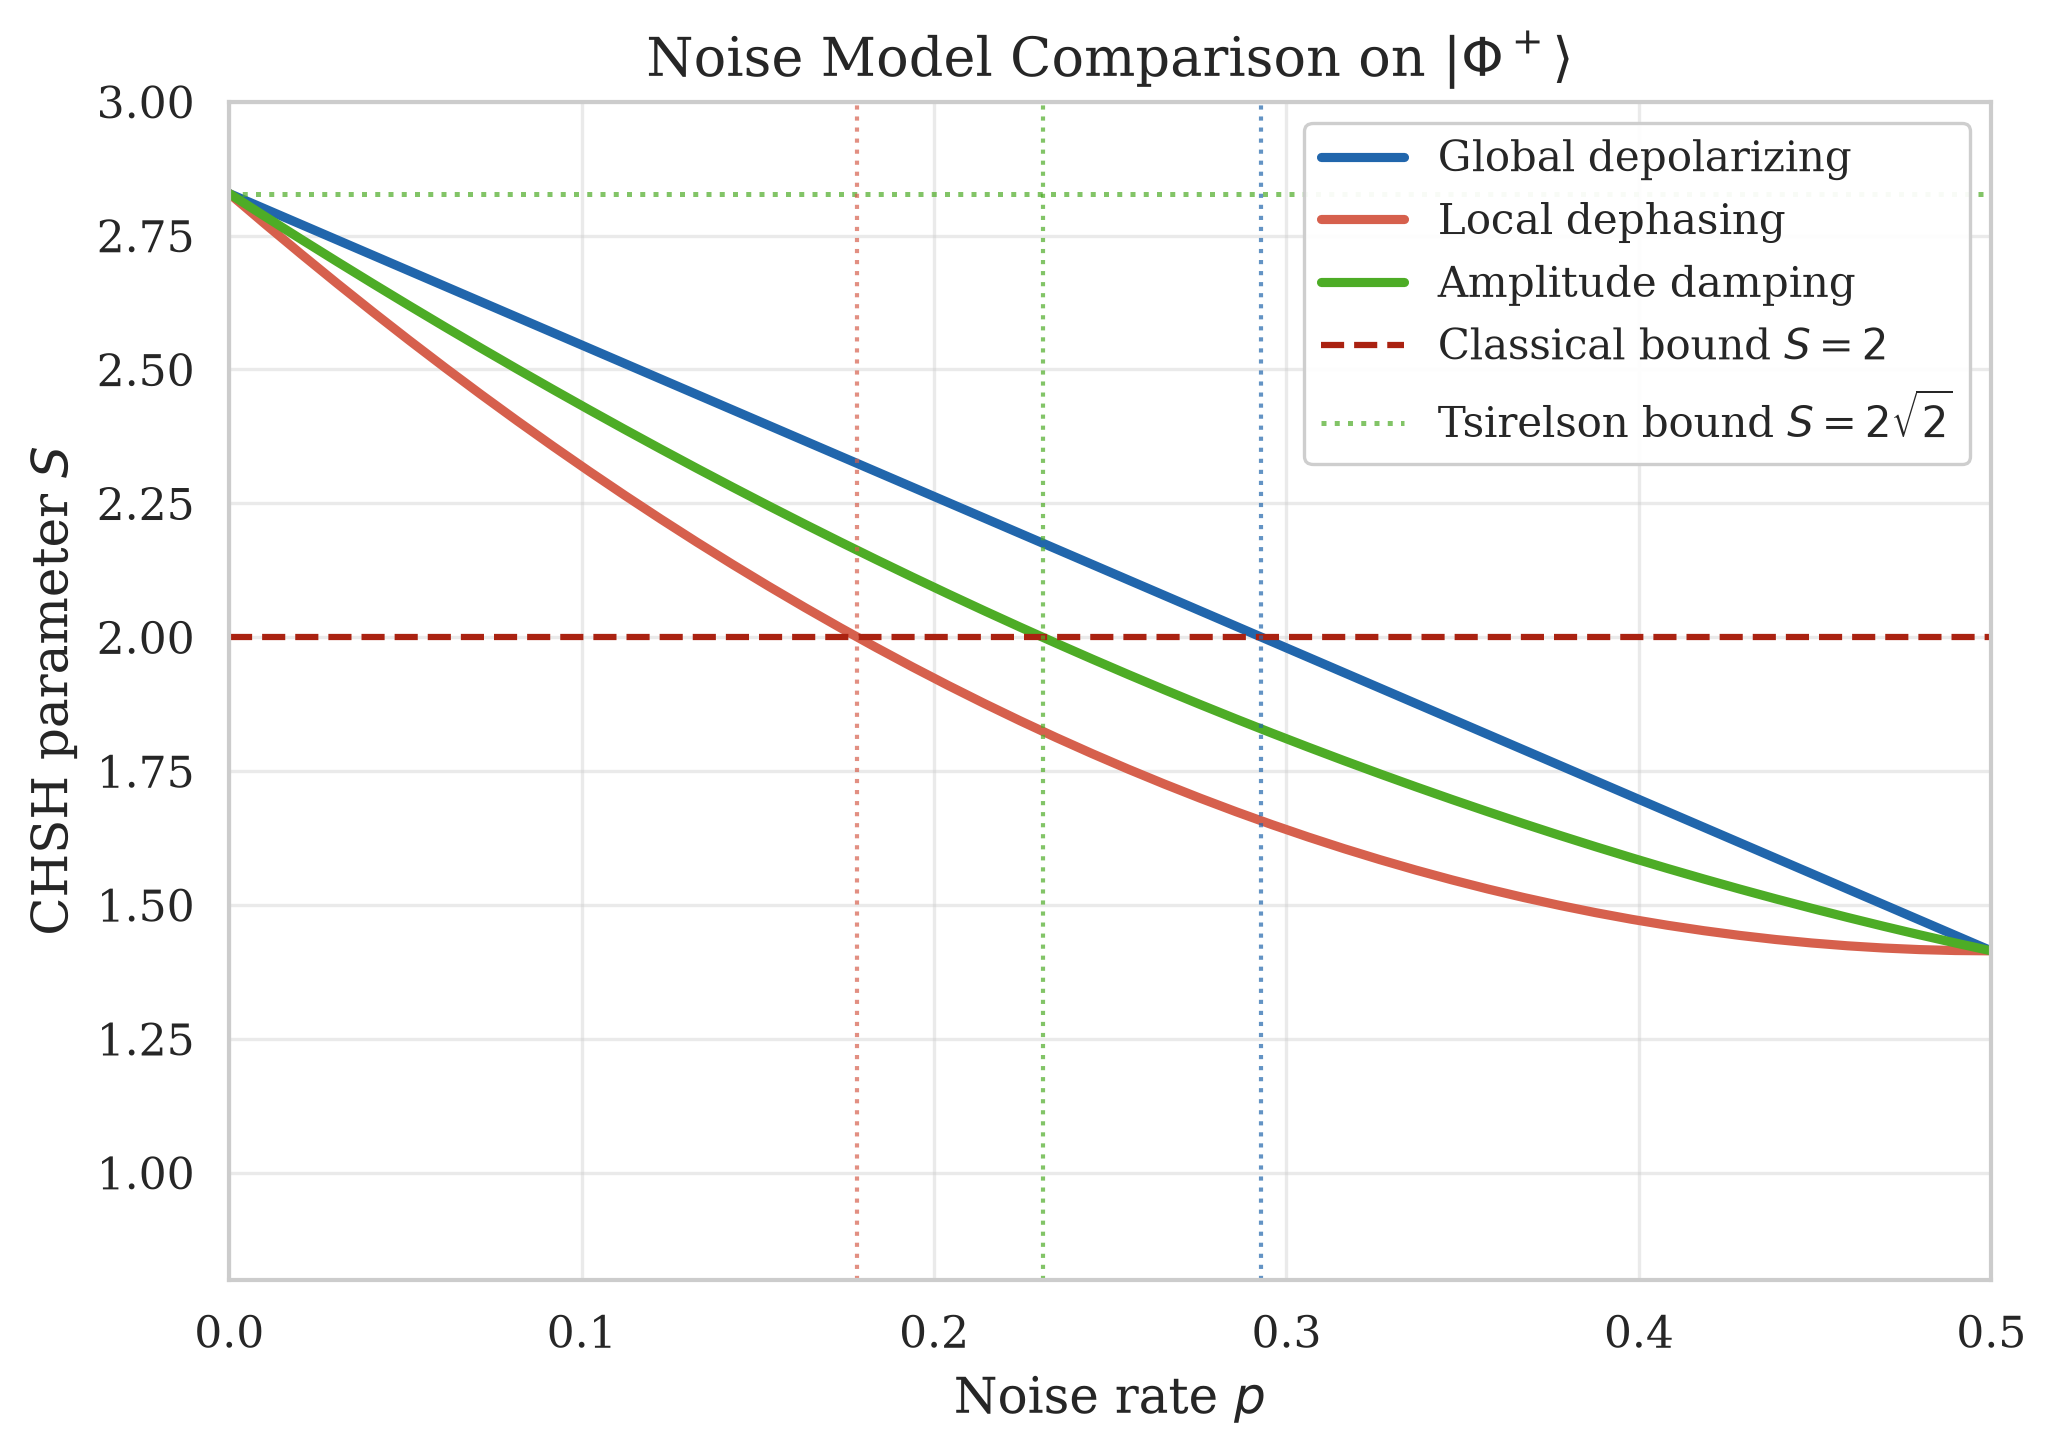
\includegraphics[width=0.75\textwidth]{figures/fig3_noise_comparison.png}
  \caption{CHSH parameter $\bigS$ versus noise rate for three noise models applied to $\Phiplus$.
           Global depolarizing (blue), local dephasing (orange), and amplitude damping (green).
           Horizontal dashed line: classical bound $\bigS = 2$.
           Dephasing and amplitude damping reach the classical bound at strictly lower noise rates,
           demonstrating their greater destructive effect on Bell correlations.}
  \label{fig:noise_comparison}
\end{figure}

\subsection{Bell State Symmetry}
\label{subsec:res_bell_states}

Under global depolarizing noise, all four Bell states trace out identical $\bigS(p)$ curves
(Figure~\ref{fig:bell_states}), sharing the threshold $\pstar \approx 0.2929$.
This is a structural consequence of the channel's local-unitary invariance: $U(\Id/4)U^\dagger = \Id/4$
for any unitary $U$, so the channel commutes with all local operations $U_A \otimes U_B$.
Since the four Bell states are related by exactly such local unitaries
($\Phiminus = (Z\otimes\Id)\Phiplus$, $\Psiplus = (X\otimes\Id)\Phiplus$, and so on),
depolarizing noise cannot distinguish among them.
Each state has its own optimal measurement angles, but the CHSH value and its noise dependence
are identical across all four.

\begin{figure}[H]
  \centering
  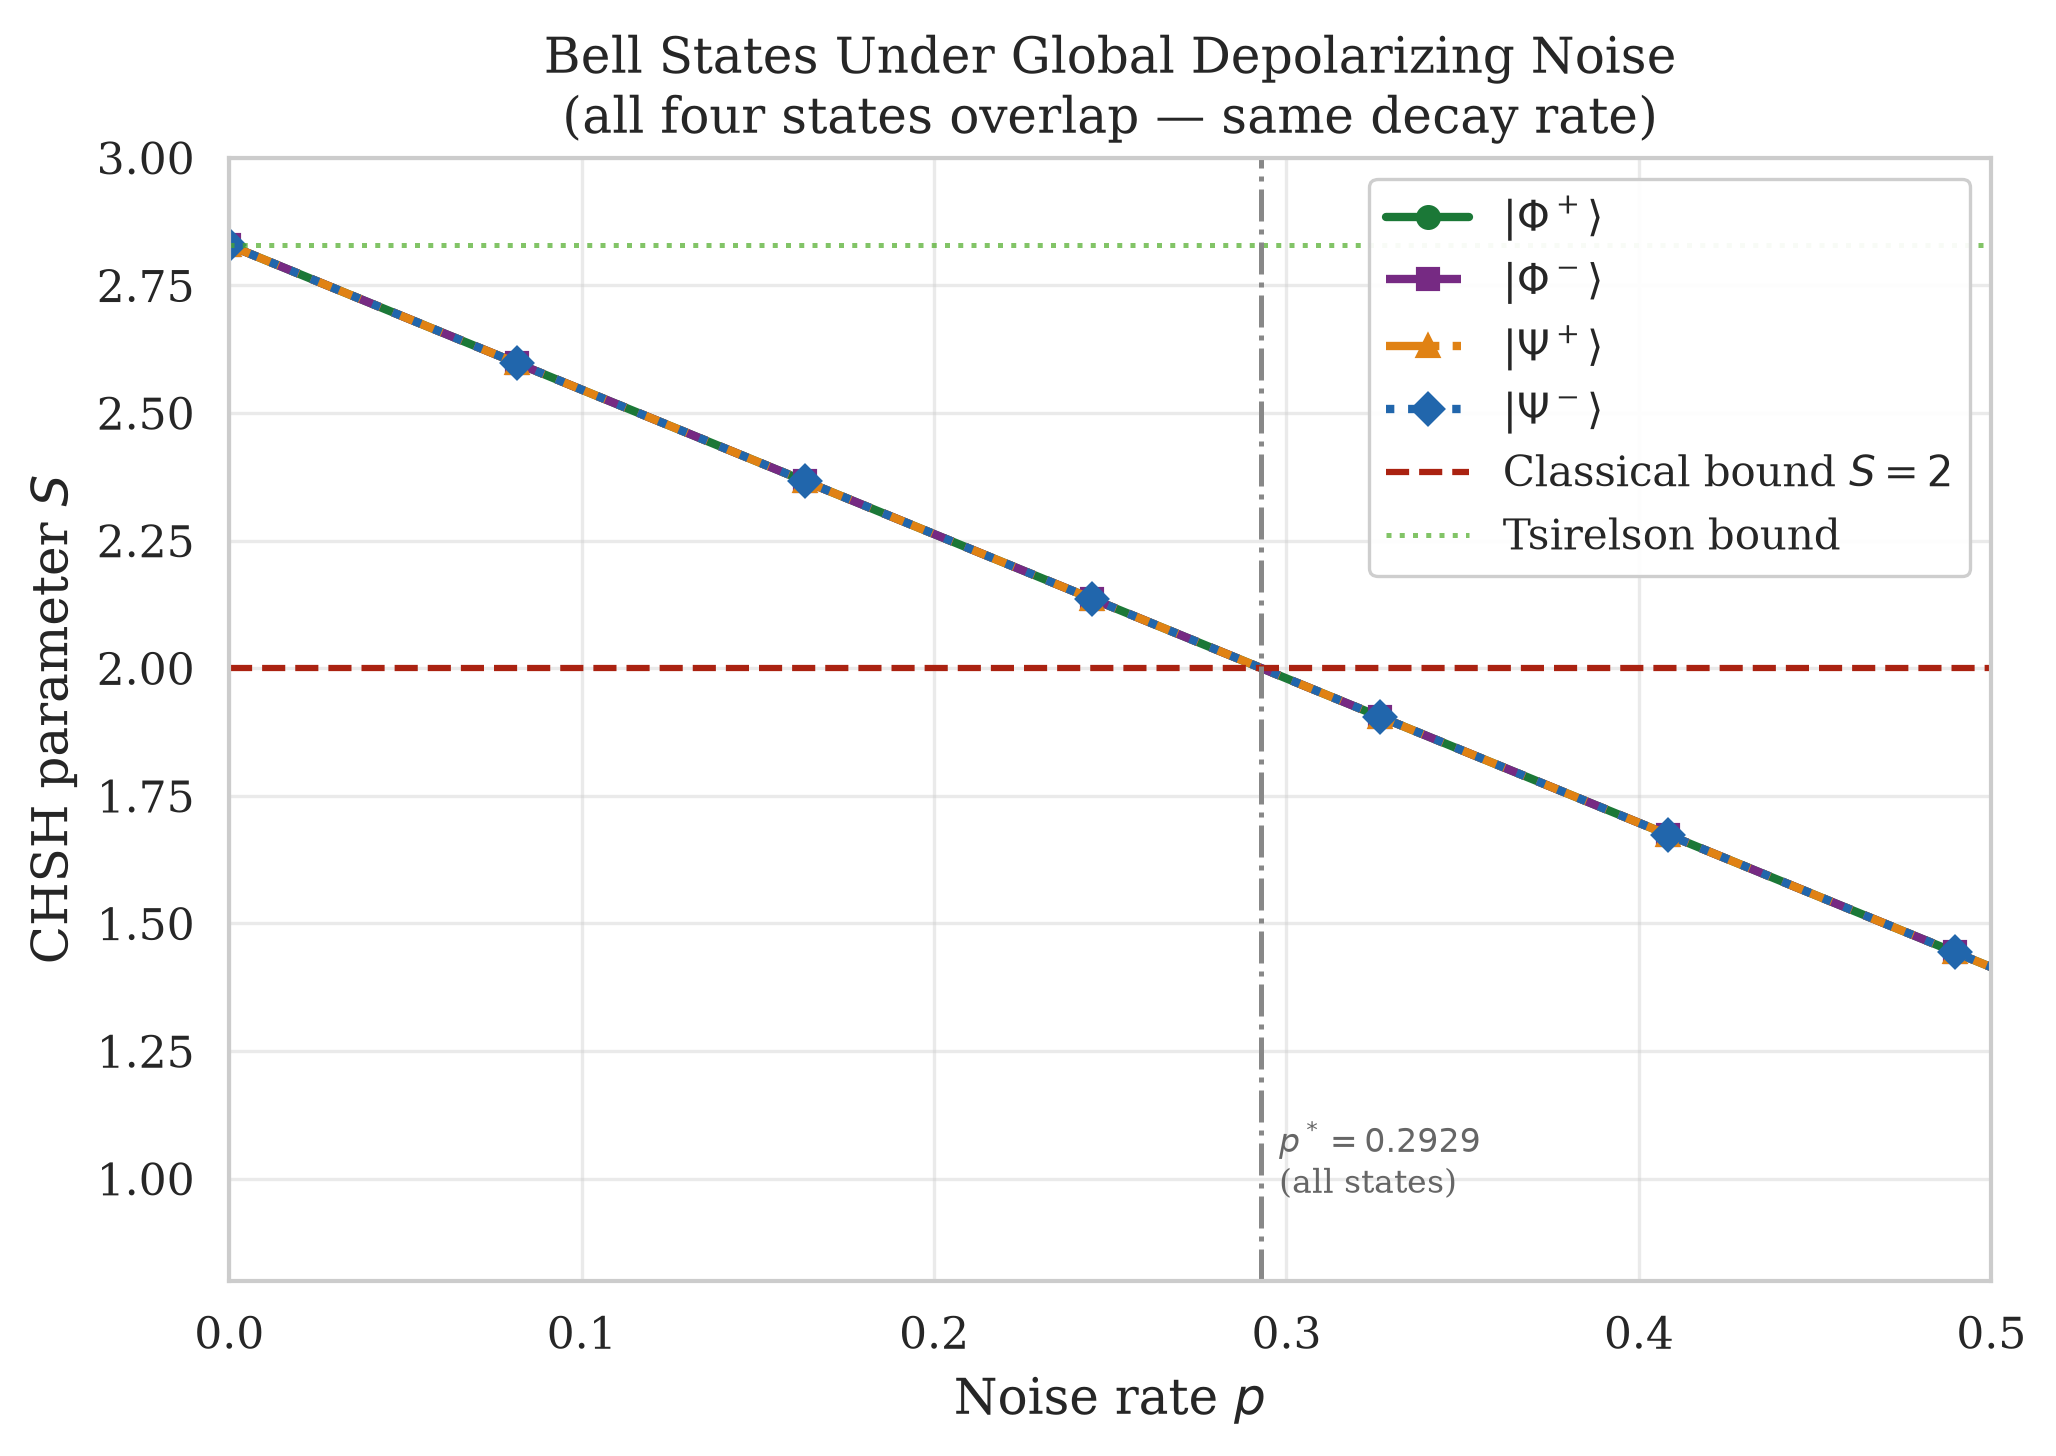
\includegraphics[width=0.75\textwidth]{figures/fig4_bell_states.png}
  \caption{CHSH parameter $\bigS$ versus depolarizing noise rate for all four Bell states
           ($\Phiplus$, $\Phiminus$, $\Psiplus$, $\Psiminus$).
           All four curves are superimposed, confirming that the decoherence threshold
           $\pstar \approx 0.2929$ is universal across Bell states under symmetric noise.}
  \label{fig:bell_states}
\end{figure}

\subsection{Measurement Angle Robustness}
\label{subsec:res_angles}

Figure~\ref{fig:angle_heatmap} maps $\bigS$ over the full two-dimensional space of Alice's
measurement angles $(\theta_A, \theta_{A'})$, with Bob's settings held at their optimal values
$b = \pi/4$, $b' = 3\pi/4$ and $p=0$.
The maximum $2\sqrt{2}$ is reached at $(a, a') = (0, \pi/2)$, confirming
equation~\eqref{eq:optimal_angles}; the surrounding landscape is a smooth plateau rather than a sharp peak.
To leading order in an angular perturbation $\delta\theta$,
\begin{equation}
  \bigS(\delta\theta) \approx 2\sqrt{2}\cos(\delta\theta) \approx 2\sqrt{2}\left(1 - \frac{\delta\theta^2}{2}\right),
  \label{eq:angle_perturb}
\end{equation}
so a $5^\circ$ misalignment reduces $\bigS$ by only $0.4\%$.
Angular errors do not shift the decoherence threshold: because both the noisy $\bigS(p)$
and the CHSH boundary scale by the same geometric factor, the crossing $\bigS = 2$ occurs at
the same $p$ regardless of small perturbations.
In practice, this means angle calibration errors do not appreciably reduce the usable noise budget.

\begin{figure}[H]
  \centering
  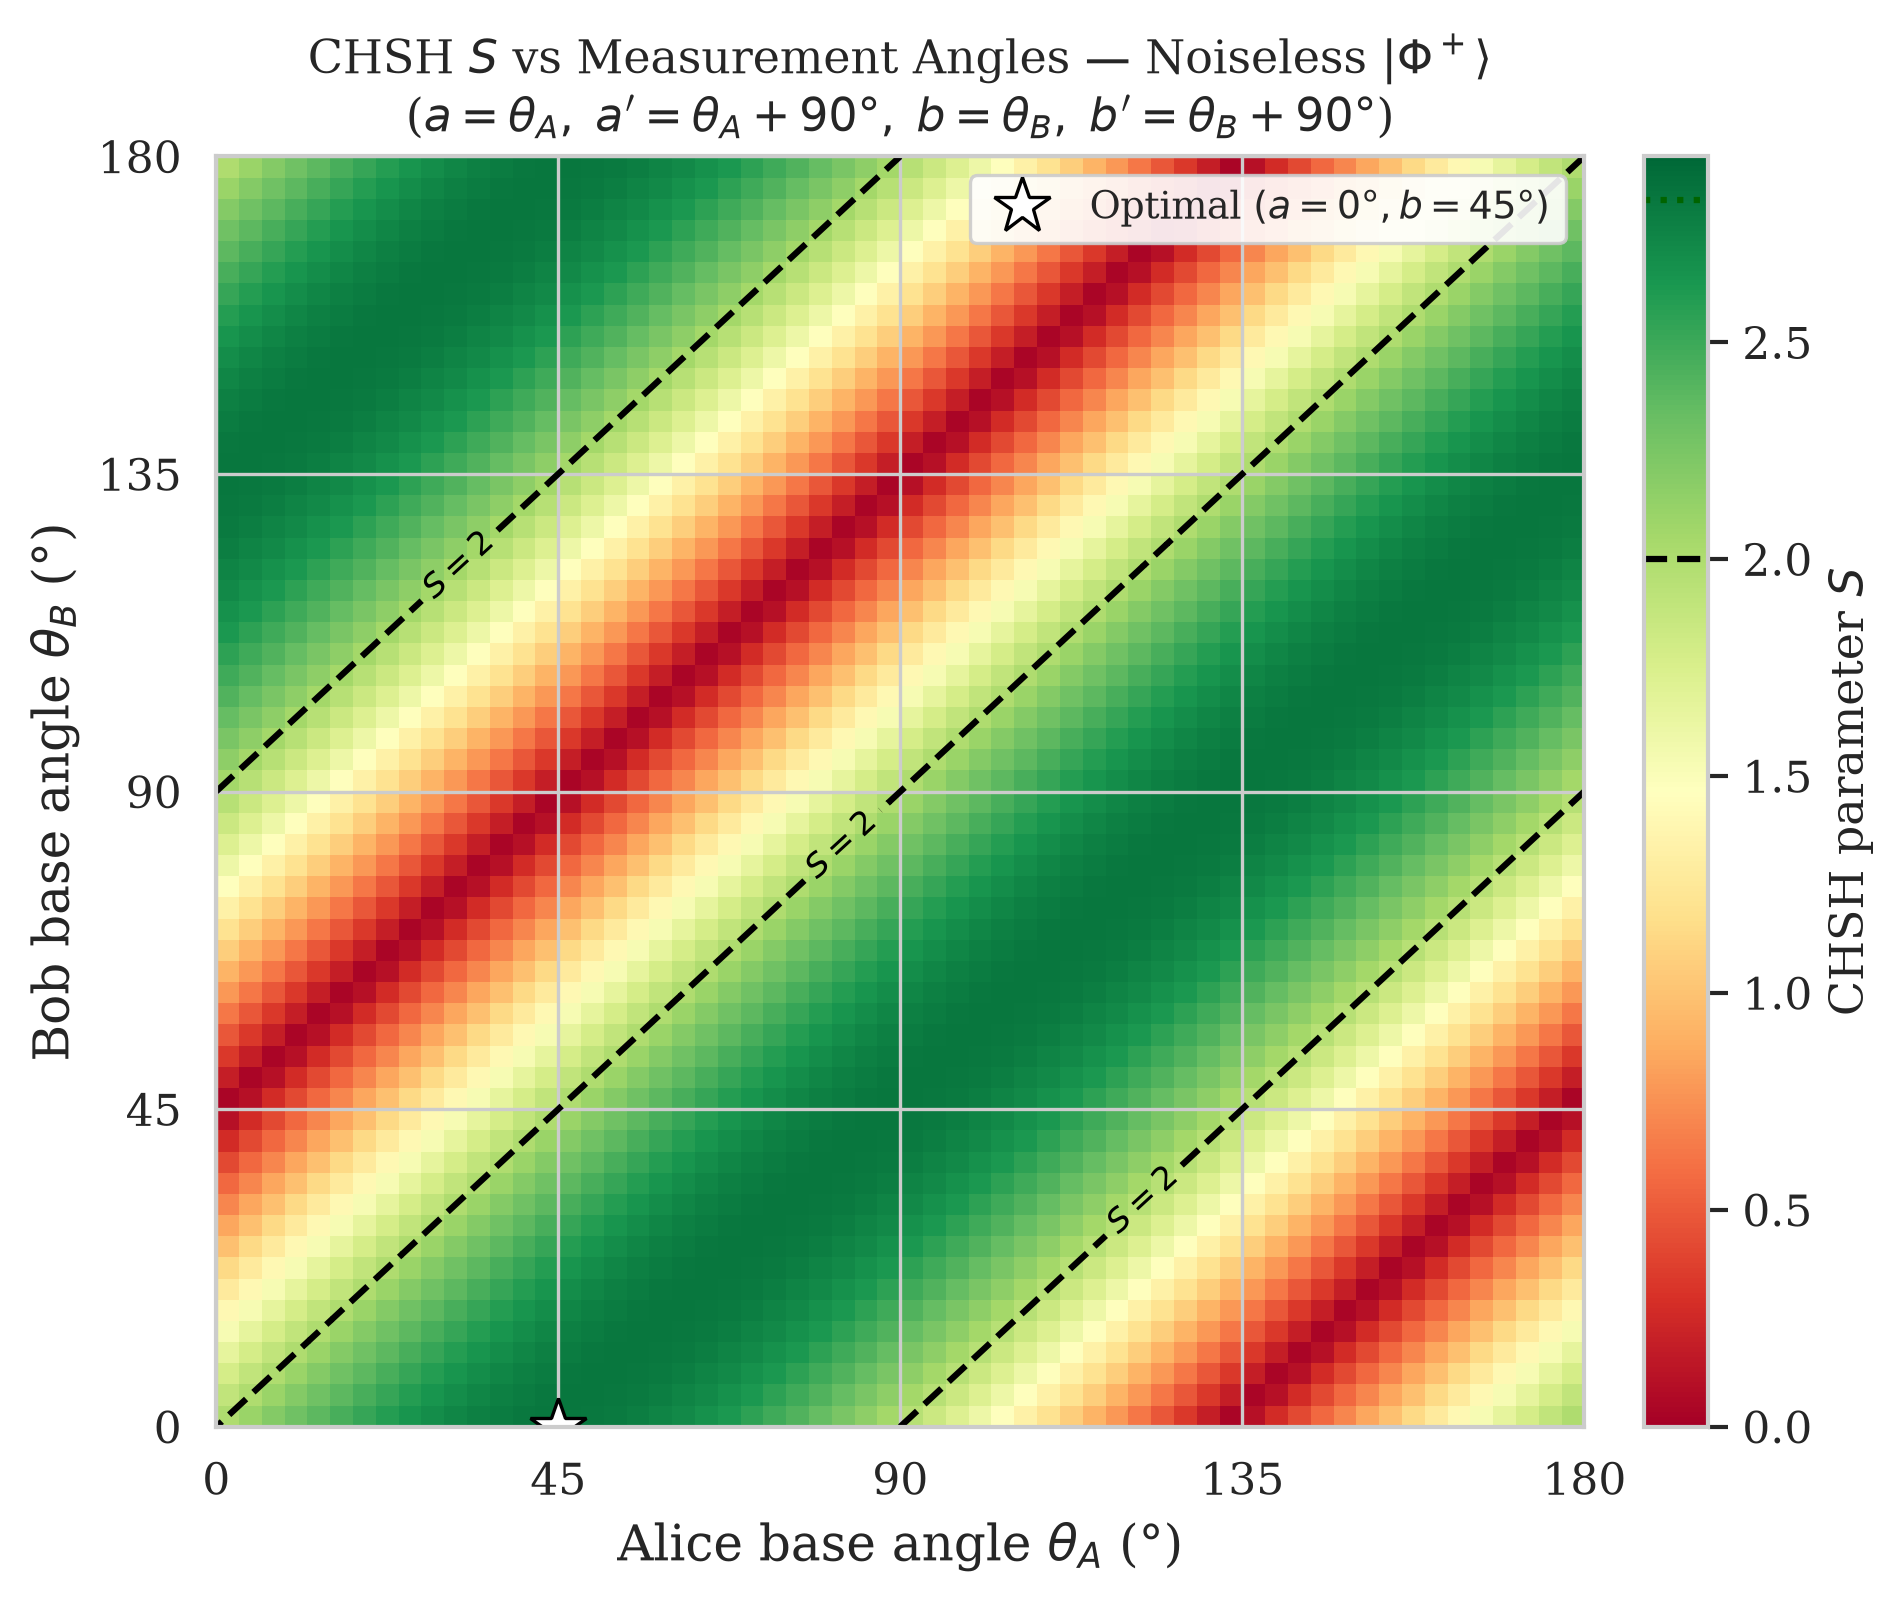
\includegraphics[width=0.65\textwidth]{figures/fig5_angle_heatmap.png}
  \caption{Heatmap of CHSH parameter $\bigS$ as a function of Alice's measurement angles
           $\theta_A$ (horizontal) and $\theta_{A'}$ (vertical), with Bob's angles fixed
           at optimal values ($b = \pi/4$, $b' = 3\pi/4$) and $p = 0$.
           The maximum $2\sqrt{2}$ is achieved at $\theta_A = 0$, $\theta_{A'} = \pi/2$.
           The white contour marks $\bigS = 2$ (CHSH boundary).}
  \label{fig:angle_heatmap}
\end{figure}

\begin{figure}[H]
  \centering
  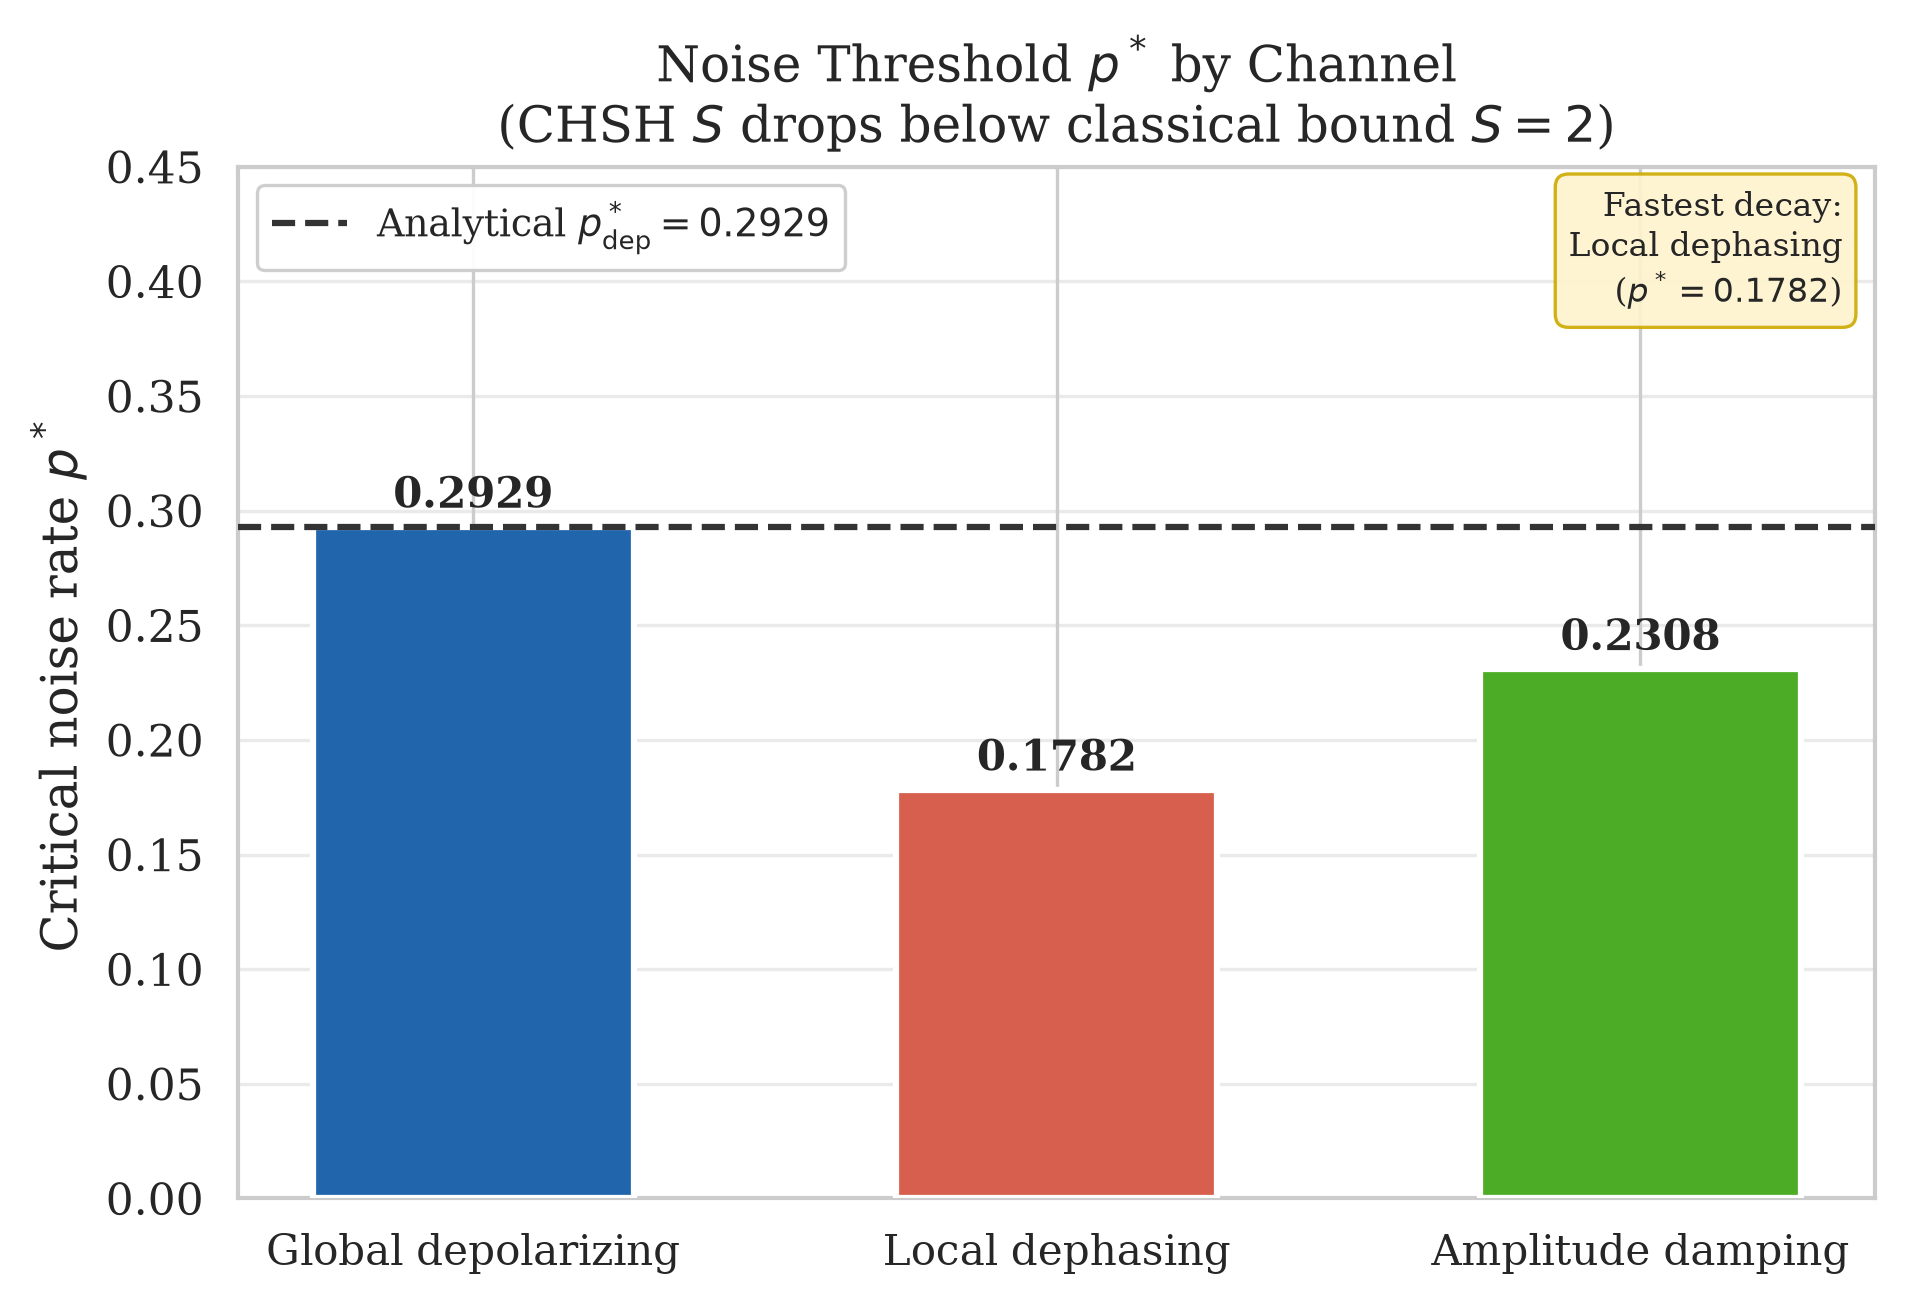
\includegraphics[width=0.65\textwidth]{figures/fig6_thresholds.png}
  \caption{Bar chart comparing the decoherence threshold $\pstar$ for three noise models.
           Global depolarizing has the highest threshold ($\approx 0.293$), followed by
           amplitude damping ($\approx 0.231$) and local dephasing ($\approx 0.178$).
           A lower threshold indicates that the noise model is more destructive to Bell correlations.}
  \label{fig:threshold_comparison}
\end{figure}

% ============================================================
\section{Discussion}
\label{sec:discussion}
% ============================================================

\subsection{Physical Interpretation of the Threshold}
\label{subsec:discuss_physical}

Above $\pstar \approx 0.293$, no choice of measurement angles can recover CHSH-violating
correlations from a depolarized Bell state; the boundary is not an artifact of a suboptimal
strategy. The Werner state characterization makes this precise: for $w = 1-p \leq 1/\!\sqrt{2}$,
Werner showed directly that a local hidden-variable model exists~\cite{werner1989}.
The regime $w \leq 1/3$ is also separable, so entanglement is destroyed at even lower noise,
though entanglement can survive without violating any Bell inequality~\cite{horodecki2009}.

Connecting $\pstar$ to hardware requires care about what $p$ represents: here it parametrizes
the full two-qubit channel, not a per-gate error.
IBM Eagle~R3 processors report two-qubit gate error rates of $\varepsilon_{2Q} \approx 0.5\%$~\cite{bharti2022noisy},
so a Bell state prepared with a single CNOT accumulates $p \approx 0.005$, roughly $60\times$
below the threshold.
Single Bell tests on current superconducting hardware are therefore straightforward, consistent
with the near-unity CHSH violations already demonstrated experimentally.
The threshold becomes relevant when circuits accumulate noise across many gates.

\subsection{Implications for Multi-Qubit Circuit Depth}
\label{subsec:discuss_depth}

For a GHZ state $(\ket{0}^{\otimes n} + \ket{1}^{\otimes n})/\sqrt{2}$ prepared with $n-1$
sequential CNOT gates, each contributing independent depolarizing noise at rate $\varepsilon_{2Q}$,
the effective noise rate on the prepared state grows as
\begin{equation}
  p_{\rm eff} \approx 1 - (1-\varepsilon_{2Q})^{n-1} \approx (n-1)\varepsilon_{2Q}
  \label{eq:accumulated_noise}
\end{equation}
for small $\varepsilon_{2Q}$.
Setting $p_{\rm eff} = \pstar$ gives a critical circuit depth of
\begin{equation}
  n^* \approx \frac{\pstar}{\varepsilon_{2Q}} + 1 \approx \frac{0.293}{0.005} + 1 \approx 60 \text{ gates}.
  \label{eq:critical_depth}
\end{equation}
Circuits exceeding roughly 60 two-qubit gates on current Eagle~R3 hardware will have accumulated
enough depolarizing noise to eliminate CHSH-certifiable entanglement, setting a concrete depth
limit for variational algorithms that rely on entanglement to achieve quantum advantage~\cite{bharti2022noisy}.
This estimate is optimistic: it neglects idling decoherence from $T_1$ and $T_2$, readout error,
and cross-talk, all of which would tighten the bound further.
The dephasing and amplitude damping thresholds derived here ($\pstar \approx 0.178$ and
$0.231$, respectively) suggest that idle-time noise during gate scheduling reduces the effective
depth limit to somewhere between 36 and 46 gates, a more realistic ceiling for circuits
interleaved with wait times.

\subsection{Connection to Quantum Key Distribution}
\label{subsec:discuss_qkd}

Device-independent QKD~\cite{acin2007} makes the stakes concrete.
DI-QKD security proofs do not assume anything about the internal workings of Alice's and Bob's
devices; they require only that the parties observe $\bigS > 2$.
Our result translates this into a channel noise budget: any link introducing more than
$\approx 29.3\%$ global depolarizing noise makes DI-QKD impossible in principle.
The tighter thresholds for dephasing ($\approx 0.178$) and amplitude damping ($\approx 0.231$)
mean that the choice of noise model matters when specifying channel fidelity requirements.
A protocol designer who assumes depolarizing noise but operates on a dephasing-dominated channel
would overestimate the permissible noise budget by nearly $65\%$.

These results also connect to the broader hierarchy of quantum correlations reviewed in~\cite{brunner2014}.
CHSH violation certifies nonlocality stronger than quantum steering, which is in turn stronger
than entanglement. The noise rates derived here therefore sit at the top of that hierarchy:
they are lower bounds on the noise rates at which weaker correlation witnesses would also fail.

% ============================================================
\section{Conclusion}
\label{sec:conclusion}
% ============================================================

How much global depolarizing noise can a Bell state absorb before it can no longer certify
nonlocality? The threshold is $\pstar = 1 - 1/\sqrt{2} \approx 0.2929$, and it is exact rather
than a fitted value. The reason is a simple algebraic fact: Pauli tracelessness forces the
maximally mixed state to contribute nothing to any correlator.
The same reasoning connects to Werner's 1989 analysis: the depolarized Bell state is a Werner
state, and Theorem~\ref{thm:depol} reproduces Werner's violation criterion by an elementary route,
with the two derivations cross-checking each other.

Comparing noise models reveals structure that the depolarizing case alone cannot show.
Local dephasing targets the off-diagonal density matrix elements that carry CHSH correlations,
pushing the threshold down to $\pstar \approx 0.178$, some $40\%$ below the depolarizing value.
Amplitude damping, which breaks exchange symmetry and produces a nonlinear decay profile,
falls between the two at $\pstar \approx 0.231$.
On superconducting hardware, these numbers translate into depth limits: roughly 60 two-qubit
gates under depolarizing-dominated gate noise, dropping to around 36 gates when idle-time
dephasing dominates.
The noise model is not an academic choice; it sets the noise budget for a given device and
circuit architecture.
\begin{equation}
  \pstar = 1 - \frac{1}{\sqrt{2}} \approx 0.2929.
  \label{eq:pstar_final}
\end{equation}

Several extensions follow naturally.
The same question for multipartite states (GHZ, graph states, resource states for
measurement-based quantum computation) remains largely open analytically; the tracelessness
argument and Werner state connection may generalize, but the richer structure of multipartite
Bell inequalities (Mermin, Svetlichny) introduces subtleties that warrant separate treatment.
The analysis also assumes Markovian noise; non-Markovian backaction, relevant on timescales
comparable to the bath correlation time in some superconducting systems, would modify the
effective noise rate in ways the simple channel model cannot capture.
Finally, translating these thresholds into concrete error-mitigation overhead, specifically
how many zero-noise extrapolation samples are needed to recover a CHSH-violating signal from
a circuit operating above $\pstar$, would turn the abstract noise budget into practical resource counts.

% ---------- Acknowledgements ----------
\section*{Acknowledgements}

The authors thank the instructors and participants of QSYS 2026 at the Institute for Quantum
Computing, University of Waterloo, for stimulating discussions.
Numerical simulations were performed using Qiskit, an open-source quantum computing SDK developed
by IBM Research.

% ---------- Bibliography ----------
\bibliographystyle{unsrtnat}
\bibliography{bibliography}

% ---------- Appendix ----------
\appendix

\section{CHSH Correlator for Optimal Angles}
\label{app:correlator}

For completeness, we verify that the optimal angles~\eqref{eq:optimal_angles} yield $\bigS = 2\sqrt{2}$
for $\Phiplus$.
Using $E(\theta_A, \theta_B) = \cos(\theta_A - \theta_B)$:
\begin{align}
  E(0, \tfrac{\pi}{4})    &= \cos(-\tfrac{\pi}{4}) = \tfrac{1}{\sqrt{2}}, \label{eq:e1}\\
  E(0, \tfrac{3\pi}{4})   &= \cos(-\tfrac{3\pi}{4}) = -\tfrac{1}{\sqrt{2}}, \label{eq:e2}\\
  E(\tfrac{\pi}{2}, \tfrac{\pi}{4})  &= \cos(\tfrac{\pi}{4}) = \tfrac{1}{\sqrt{2}}, \label{eq:e3}\\
  E(\tfrac{\pi}{2}, \tfrac{3\pi}{4}) &= \cos(-\tfrac{\pi}{4}) = \tfrac{1}{\sqrt{2}}. \label{eq:e4}
\end{align}
Therefore,
\begin{equation}
  \bigS = \left|E(0,\tfrac{\pi}{4}) - E(0,\tfrac{3\pi}{4}) + E(\tfrac{\pi}{2},\tfrac{\pi}{4}) + E(\tfrac{\pi}{2},\tfrac{3\pi}{4})\right|
        = \left|\tfrac{1}{\sqrt{2}} + \tfrac{1}{\sqrt{2}} + \tfrac{1}{\sqrt{2}} + \tfrac{1}{\sqrt{2}}\right|
        = 2\sqrt{2}. \label{eq:smax_verify}
\end{equation}

\section{Local Dephasing: Analytical Treatment}
\label{app:dephasing}

For local dephasing with rate $p$ applied to both qubits, the two-qubit channel acts as
\begin{equation}
  \rho \;\mapsto\; \sum_{i,j \in \{0,1\}} p^{(i+j)/2}(1-p)^{(2-i-j)/2}\,(Z^i\otimes Z^j)\,\rho\,(Z^i\otimes Z^j),
  \label{eq:dephase_twoqubit}
\end{equation}
where the sum runs over $i,j \in \{0,1\}$ indexing which qubits are affected.
One can show that the off-diagonal density matrix elements acquire a suppression factor $(1-2p)^2$,
giving
\begin{equation}
  E_{\rm deph}(\theta_A,\theta_B) = (1-2p)^2\cos(\theta_A - \theta_B)
  \label{eq:e_dephased}
\end{equation}
for the components involving $\sigma_x$ and $\sigma_y$.
Setting $\bigS_{\rm deph}(p) = (1-2p)^2\cdot 2\sqrt{2} = 2$ yields
\begin{equation}
  \pstar_{\rm deph} = \frac{1}{2}\!\left(1 - \frac{1}{\sqrt[4]{2}}\right) \approx 0.2071,
  \label{eq:pstar_deph}
\end{equation}
though this expression assumes the simplest single-qubit dephasing model and the exact numerical
value depends on the specific channel parametrization adopted in the simulation.

\end{document}
